\chapter{Обзор методов обучения с подкреплением и их применения в роботике}\label{ch:ch1}

Машинное обучение с подкреплением строится на взаимодействии агента со средой. Средой в зависимости от решаемой задачи может являться компьютерная игра, мир окружающий робота или физическая установка. Граница разделяющая агента и среду достаточно условна. В качестве примера можно рассмотреть робот-манипулятор. Если агент непосредственно управляет положением суставов манипулятора, то суставы является частью агента. Если же агент задает конечное положение захвата манипулятора, а положение составов вычисляется с помощью встроенного алгоритма, то суставы манипулятора являются частью среды. 

Агент взаимодействует со средой посредством  действий из заранее заданного набора $a \in \mathcal{A}$. При каждом взаимодействии среда переходит в новое состояние $s \in \mathcal{S}$, а агент получает награду $r \in \mathcal{R}$.
Цель обучения агента заключается в нахождении последовательности действий при которой агент получит максимальную суммарную награду. 

\section{Обзор методов глубокого обучения с подкреплением}\label{sec:ch1/sec1}

Глубокое обучение с подкреплением основано на объединении нейронных сетей и методов обучения с подкреплением. Нейронная сеть выступает в качестве универсального аппроксиматора и определяет стратегию агента при взаимодействии со средой $\pi_{\theta}$.

\subsection{Нейронные сети}

Понятие искусственной нейронной сети было впервые предложено У. Маккалоком и У. Питтсом в 1943 году в работе "Логическое исчисление идей, относящихся к нервной активности" \cite{McCulloch1943}. Первая нейронная сеть с одним скрытым слоем, пороговой функцией активации и прямым распространением сигнала была предложена Ф. Розенблаттом в 1957 году \cite{rosenblatt}.

\begin{figure}[ht]
	\centerfloat{
		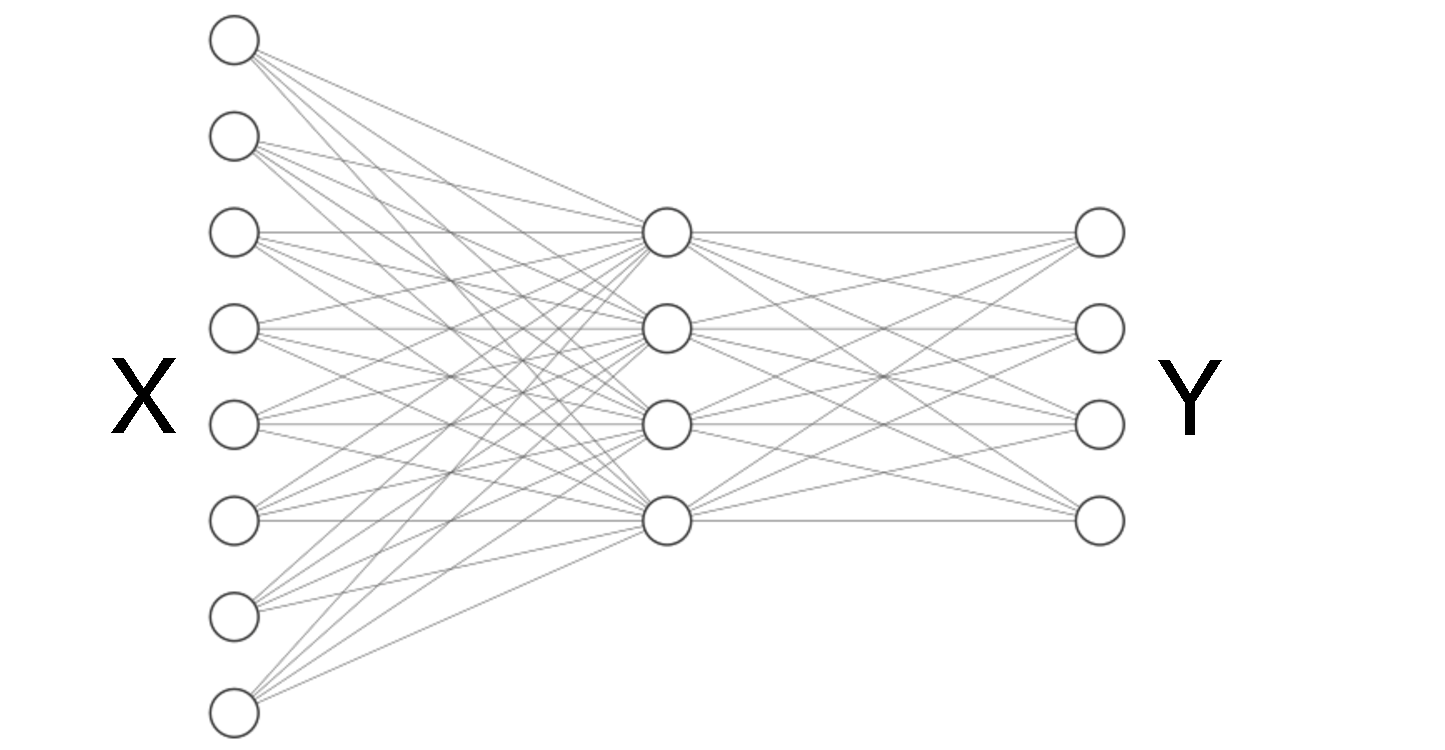
\includegraphics[width=0.7\linewidth]{images/fcnn}
	}
	\caption{Полносвязная нейронная сеть с одним скрытым слоем}
	\label{fig:fcnn}
\end{figure}

Схематически полносвязная нейронная сеть с одним скрытым слоем представлена на рис. \ref{fig:fcnn}. Нейронная сеть принимает на вход вектор входных параметров $X$ и возвращает на выходе вектор выходных параметров $Y$. Значение в нейроне на слое $i$ вычисляется как взвешенная сумма значений нейронов на слое $i - 1$. Для оптимизации (обучения) параметров нейросети применяется алгоритм обратного распространения ошибки, который был одновременно разработан А.И. Галушкиным \cite{Galushkin} и П.Д.Вебросом \cite{webros_1974}. На каждой итерации алгоритма \ref{alg:backprop} происходит два прохода - прямой и обратный. Во время прямого прохода ($X \to Y$) вычисляются выходные значения при прохождении входного вектора от входов сети к выходам. Затем во время обратного прохода ошибка предсказания для слоя $i$ вычисляется на основе ошибки для слоя $i + 1$ и обновление весов производится с помощью метода градиентного спуска. 

\begin{algorithm}[ht]
	\SetAlgoLined
	\KwIn{$X$ - входные наблюдения, $\hat{Y}$ - ожидаемые выходные значения, $L(Y, \hat{Y})$ - функция потерь, $W$ - параметры нейронной сети}
	\KwOut{$W^{\prime}$ - новые значения параметров нейронной сети}
	\While{$L(Y, \hat{Y})$ > $\varepsilon$}{
		Выбираем $x \sim X$, $\hat{y} \sim \hat{Y}$\;
		Прямой проход: y = NN(W, x)\;
		Вычисляем ошибку предсказания: $E = L(y, \hat{y})$\;
		Обратный проход: $\Delta w_{ij} = -\eta \frac{\partial E}{\partial w_{ij}}$\;
		$S_j = \sum_{i = 1}^{n}w_{ij}x_i$\;
		$\frac{\partial E}{\partial w_{ij}} = \frac{\partial E}{\partial S_j}\frac{\partial S_j}{\partial w_{ij}} = x_i\frac{\partial E}{\partial S_j}$\;
		
	}
	\caption{Алгоритм обратного распространения ошибки}
	\label{alg:backprop}

\end{algorithm}

Нейронная сеть с достаточно большим количеством параметров может выступать в качестве универсального аппроксиматора. Доказательством этого является теорема Колмогорова-Арнольда\cite{kolmogorov, arnold}: многомерная функция многих переменных может быть представлена в виде суперпозиции непрерывных функций одной переменной. 


\subsection{Обучение с подкреплением}

Принципиальная схема обучения RL алгоритмов приведена на рисунке \ref{fig:rl}. На ней агент получает от среды состояние (s $\in \mathcal{S}$), награду ($r: \mathcal{S} \times \mathcal{A} \to \mathbb{R}$), и флаг завершения эпизода (done $\in \{0, 1\}$).  В среде агент совершает действие ($a \in \mathcal{A}$) которое переводит среду в следующее состояние ($s^{\prime} \in \mathcal{S}$). В зависимости от того является ли переход из состояния $s$ в состояние $s^{\prime}$ при действии $a$ единственным или одним из возможных с вероятностью $p(s^{\prime},r|s,a)$, среда называется детерминированной или не детерминированной. 

\begin{figure}[ht]
	\centerfloat{
		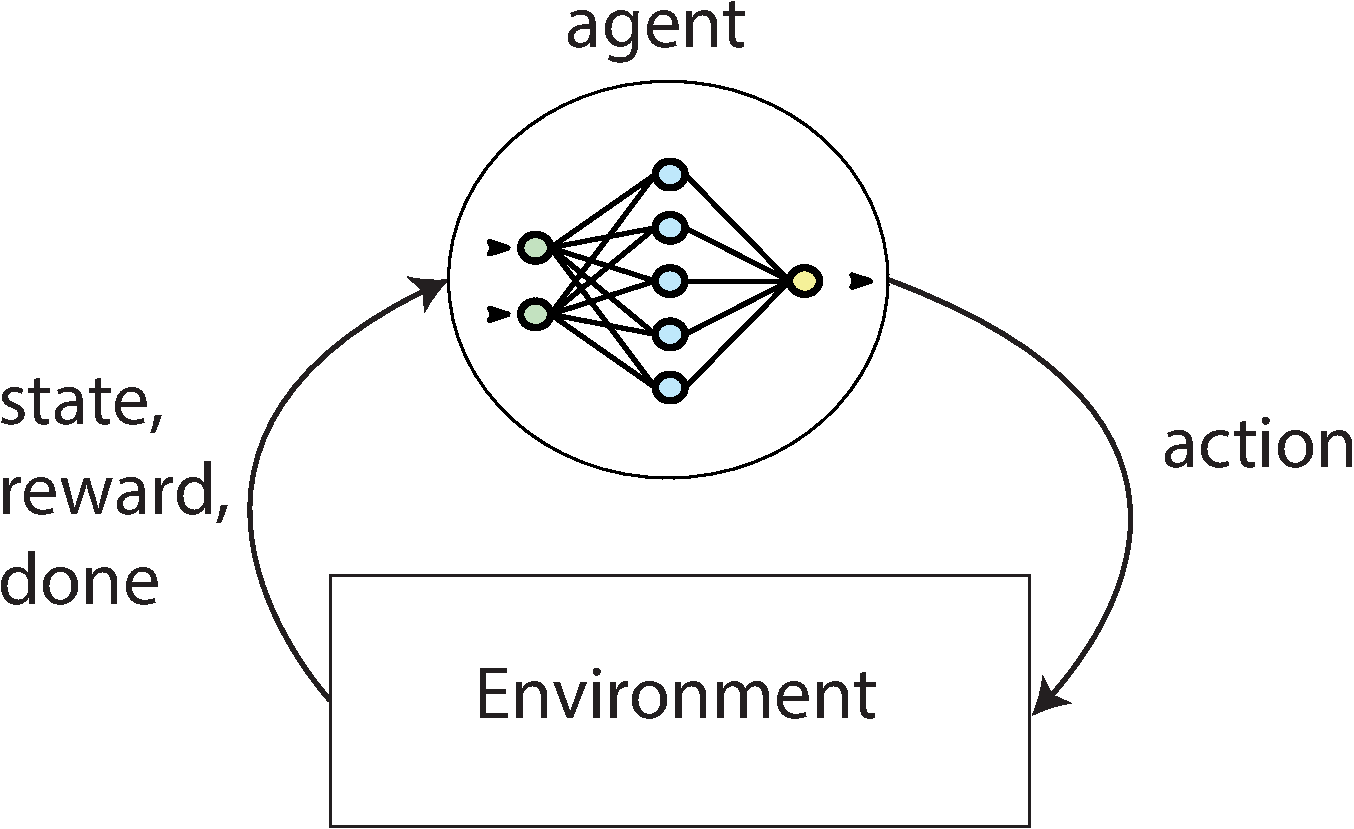
\includegraphics[width=0.5\linewidth]{images/rl_setting}
	}
	\caption{Взаимодействие агента и среды}
	\label{fig:rl}
\end{figure}

Процесс работы RL агента строится на марковском процессе принятия решений (МППР). В нем предполагается, что следующее состояние и награда которую получит агент зависит только от предыдуюего состояния и действия которое агент совершил. Если же у среды есть некоторые не наблюдаемые параметры, то говорят о частично наблюдаемом марковском процессе принятия решений (ЧНМППР). В нем наблюдение в момент времени $t$ --- $o_t \in \mathcal{O}$ определяется распределением $o_t \sim U(o_t|s_t)$, где $s_t \in \mathcal{S}$ полное состояние среды. 

Стратегия агента является детерминированной функцией $a_t=\pi(s_t)$ отображающей пространство состояний (наблюдений) в пространство действий $\mathcal{A}$. Задача агента состоит в максимизации суммарной ожидаемой дисконтированной награды к концу эпизода:

\begin{equation}
\ex_{\tau \sim \pi_{\theta}} [J(\tau)] = \ex_{\tau \sim \pi_{\theta}} [r_0 + \gamma r_{1} + \gamma ^ 2 r_{2} + ...] = \ex_{\tau \sim \pi_{\theta}} [\sum_{t} \gamma ^t r_{t}]
\end{equation}

Коэффициент $\gamma \in (0, 1]$ вводится для  ограничения эффективного горизонта --- числа шагов при котором будущая награда не влияет на политику из-за дисконтирования ($\gamma ^ n r$). 
Он также позволяет регулировать уровень жадности агента --- на сколько награда получаемая на текущем шаге ценнее аналогичной награды получаемой на следующем шаге. Математическое ожидание берется по траекториям $\tau$ полученным с помощью текущей стратегии $\pi_{\theta}$ параметризованной весами $\theta$. 
Вероятность траектории $\tau$ может быть записана следующим образом:
 
 \begin{equation}
     p(\tau|\pi) = p(s_0) \prod^T_{t=1}p(s_t|s_{t-1}, a_{t-1})\pi(a_{t-1}, s_{t-1})
\end{equation}

 где $p(s_0)$ - распределение начальных состояний в каждом эпизоде, $p(s_t|s_{t-1}, a_{t-1})$ - распределение описывающее динамику среды.
 
 Таким образом для задания среды необходимо определить $<\mathcal{S, R, A, P}, \gamma>$.


\subsection{Уравнение Беллмана}

Ценность нахождения агента в состоянии $s_t$ описывается с помощью V-функции и  Q-функции. $V(s_t) = \ex[\sum_{t} \gamma ^t r_{t}]$ оценивает суммарную дисконтированную награду, которую получит агент находящийся в состоянии $s_t$ если он будет следовать текущей стратегии. $Q(s_t, a_t) = \ex[r_t + \sum_{t} \gamma ^{t + 1} r_{t + 1}]$ --- суммарная дисконтированная награда, которую получит агент при совершении действия $a$ в состоянии $s_t$ и следовании дальше текущей стратегии. Значения V,Q-функций в точках $s_t$ и $s_{t + 1}$ при условии, что текущая стратегия является оптимальной связаны между собой уравнениями Беллмана: 

\begin{equation}
	V^*(s) = \max_{a \in \mathcal{A}} \ex(r_{t + 1} + \gamma V^*(s_{t + 1}))
\end{equation}

\begin{equation}
Q^*(s, a) = \ex(r_{t + 1} + \gamma \max_{a' \in \mathcal{A}} Q^*(s_{t + 1}, a'))
\end{equation}


Смысл V-функции можно легко представить в задаче изображенной на рис. \ref{fig:minigrid}. В ней агент движется из верхнего левого угла ($s_0$) сетки в правый нижний угол ($s_f$). Если агент за каждый шаг получает награду $r = -1$, то оптимальная V-функция в состоянии $s_t$ будет равна числу действий необходимых для достижения состояния $s_f$ со знаком ``-''. 

\begin{figure}[ht]
	\centerfloat{
		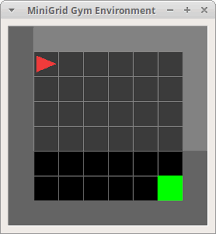
\includegraphics[width=0.3\linewidth]{images/minigrid_empty}
	}
	\caption{Среда MiniGrid-Empty-8x8-v0 \cite{gym_minigrid}}
	\label{fig:minigrid}
\end{figure}

 
\subsection{Метод value iteration}

Уравнения Беллмана могут быть использованы для построения оптимальной стратегии для сред с конечным набором состояний и известной вероятностью переходов между ними $p(s^{\prime}, r|s, a)$. Метод value iteration \ref{alg:value_it} строится на применении метода простой итерации к уравнению Беллмана для V-функции. Данный метод гарантирует сходимость \cite{Sutton1998}, но может быть использован только для очень ограниченного набора задач.

\begin{algorithm}[ht]
	\SetAlgoLined
	\KwIn{$t$ - stop threshold, $\mathcal{S}$ - set of environment states, $p(s^{\prime}, r|s, a)$ - transition probability}
	\KwOut{$\pi(s) = \mathrm{argmax}_{a} \sum_{s', r}p(s',r|s,a)[r + \gamma V(s')]$}
	Initialize V(s) = 0 (for all $s \in \mathcal{S}$)\;
	\While{$\Delta$ > t}{
		$\Delta$ = 0\;
		\ForEach{s $\in \mathcal{S}$}{
		    $V_{old}$ = V(s)\\
		    %V_{old}(s) = V(s)\par
			V(s) = $\max_a \sum_{s', r}p(s', r|s, a)[r + \gamma V(s')]$\\
			$\Delta = \max(\Delta, |V_{old} - V(s)|)$
		}
	}
	\caption{Алгоритм value iteration}
	\label{alg:value_it}

\end{algorithm}

In model-free RL, the agent learns from trial-and-error directly without any model for the reward and transitions. There are two approaches in deep RL named on-policy and off-policy diverse on data usage. In on-policy methods agent improves the policy and value function based on samples from the current policy. Policy gradients methods \cite{rl_book} e.g., TRPO \cite{trpo}, PPO \cite{ppo} learn directly policy $\pi(\cdot|s_t)$ based on the state observed under the current policy during training. In off-policy methods agent learns the optimal policy (Q-function) from replay buffer data generated by previous copies of the current policy. For example, Q-learning learns to find optimal action-value without fitting policy that generates data. Roughly speaking, off-policy and on-policy can be devised as different policy and same policy methods respectively \cite{rl_book, RL_review}. 

%TRPO \cite{trpo} is the well-known on-policy improvement of REINFORCE \cite{rl_book} based on the natural gradient approach. In our work, it’s an outer loop algorithm in the on-policy meta-learning algorithm MAML \cite{maml}. Using the Gaussian parametrization method work well in a suit of robotic continuous task (MuJoCo benchmark \cite{mujoco, mujoco_benchmark}). The main problem of on-policy algorithms is sample inefficiency compared with off-policy approaches. They sensitive to current policy and can be easily trapped by any perturbation in current policy. 

%SAC \cite{sac, sac_applications} is a state-of-the-art off-policy algorithm. It addresses learning maximum entropy policies in continuous action space. The maximum entropy objective generalizes the standard objective by augmented it with the entropy term, such that optimal policy aims to optimize entropy overall visited states. TQC \cite{tqc} gives a better solution of overestimation bias in critic networks compared to SAC. Instead of using minimum between the prediction of two nets \cite{two_nets_critic} TQC uses a distributional representation of a critic, truncation of critics predictions, and ensembling of multiple critics. %%We use TQC in our experiments.

\subsection{Off-policy алгоритмы}

\paragraph{Алгоритм DQN}
Существенной прорыв в глубоком обучении с подкреплением был достигнут в 2015 году. Авторами \cite{mnih2013atari} был разработан метод DQN который научился играть в 49 игр Atari на уровне человека. Алгоритм строится на обучении глубокой нейронной сети аппроксимировать Q-функцию для текущего состояния среды на основе изображения. 

\paragraph{Алгоритм TD3}
Существенным ограничением метода DQN является то, что он применим исключительно для сред с дискретным набором действий. 

 

The agent's objective is to learn the policy $\pi^*$ that maximizes the expected return $J(\pi) = \mathbb{E}_{\tau\sim p(\tau | \pi)}[R_0]$ where $p(\tau | \pi)$ is the distribution of trajectories $\tau = (o_0, a_0, o_1, a_1, ..., a_{T-1}, o_{T})$ produced by policy $\pi$:
\begin{equation}
    \label{eq:optEq}
    \pi^* = \argmax_{\pi}J(\pi).
\end{equation}

The agent objective is to learn policy $\pi^*$ that maximize the expected return $J(\pi) = \mathbb{E}_{\tau\sim p(\tau | \pi)}[R_0]$ where $p(\tau | \pi)$ is the likelihood of sampling trajectory $\tau = (o_0, a_0, o_1, a_1, ..., a_{T-1}, o_{T})$ having policy $\pi$.
 
 \begin{equation}
     \pi^* = \argmax_{\pi}J(\pi)
 \end{equation}
 


\textbf{Policy gradient. }
The policy $\pi$ is defined by parameters $\theta$ (i.e.~$\pi=\pi_{\theta}$), so the optimization \eqref{eq:optEq} is performed with respect to the parameters: $\theta^* = \argmax_{\theta}J(\pi_{\theta})$. A common approach to such a problem is policy gradient \citep{sutton1999policy}, which iteratively improves the policy in terms of expected return via gradient ascent:

\begin{equation}
    \theta_{t+1} = \theta_{t} + \alpha  \frac{\partial J(\pi_{\theta})}{\partial \theta},
\end{equation}

where $\alpha$ is the learning rate. The algorithms of this family vary by the method of approximating the unknown $J(\pi_\theta)$.

A common approach to continuous-action Markov decision processes is TD3 \citep{fujimoto2018addressing} which is an extension of another popular algorithm DDPG \citep{lillicrap2015continuous}. This algorithm uses three neural networks: one (actor) for a deterministic policy and two (critics) for evaluating the action-state values $Q(s_t,a_t)$. Using two critics allows the algorithm to suffer less from overestimating the Q-values; in addition, the algorithm smoothens the Q-functions by adding Gaussian noise to the target actions when updating the parameters of the critics. Gaussian noise is also added to each policy action during the training to encourage exploration.

Данный алгоритм использует нейронную сеть, определенную набором параметров $\theta$, для реализации детерминированной политики $a = \pi_{\theta}(o)$. Для обучения такой политики  функция $J(\pi_\theta)$ приближается с помощью двух Q-функций, заданных нейронными сетями что уменьшает переоценку Q-значений. 


Так TD3 использует две Q-функции вместо одной, для предотвращения переоценки $J(\pi_\theta)$, реже обновляет политику, а также сглаживает Q-функции, добавляя шум к целевому действию. 

Добавить про TD3. Exploration noise ???

что это, формулы
адвантаж, оверэстимэйшен 

\subsection{On-policy алгоритмы}

\paragraph{Алгоритм PPO}
credit assignment problem (какие действия привели к награде)
Альтернативным подходом является оптимизация стратегии на прямую. 

$$J(s) = \sum_{\pi} R(s,a )$$
$$\nabla_{\theta} J(s) = \sum_{\pi} \pi(a|s)\frac{\nabla \pi(a|s)}{\pi(a|s)}R(s,a )$$
$$\nabla_{\theta} J(s) = \sum \log(\pi(a|s))R(s,a )$$

Мотивация 
REINFORCE, Actor-Critic, PPO

The Actor network $\pi_{\theta} (\cdot|s_i)$ minimizes the following clipped objective: 

$$
L = \ex_{\tau \sim \pi_{k}} \left[ \sum_{t = 0}^{T} \min(\rho_{t}(\theta)A_t,\mathrm{clip}(\rho_t(\theta), 1 - \varepsilon, 1 + \varepsilon)A_t) \right]
$$

where $\rho_t(\theta) = \pi_{\theta}(a_t|s_t) / \pi_{\theta^{\prime}}(a_t|s_t)$ – the likelihood ratio of the action at w.r.t. the current policy and the policy used to collect the data; $A_t$ - generalized advantage estimate \cite{schulman2015high}; $\varepsilon$ - clipping parameter.

The actor’s objective is the core of the PPO algorithm \cite{schulman2017proximal}. The interplay, between the $\min$ operator, likelihood clipping, and the sign-changing multiplicative advantage $A_t$ enables controllable policy updates which mostly focus on unlikely advantageous or likely detrimental experience.

\subsection{Использование внутренней мотивации в средах с редкой наградой}
curiosity, RND , count based 

\subsection{Мета-обучение}

RL агент взаимодействует со средой во время обучения и во время тестирования. Обычно методы обучения с подкреплением предназначены для решения конкретной задачи и не могут легко обобщаться на другие похожие задачи. Для того, чтобы обучиться агента решению другой задачи его приходится начинать обучение с нуля. Таким образом для обучения многих агентов требуется существенно больше данных, что не является эффективным. 

Мета-обучение позволяет агенту научиться адаптироваться к различным задачам. В базовой постановке задачи мета-обучения рассматривается распределение задач $p(\mathcal{T})$, из которого случайным образом выбирается задача $\mathcal{T}$ в течении процесса мета-обучения. Разные задачи могут отличаться функцией награды и вероятностью переходов $p(s^{\prime}|s, a)$  из должна объединять некоторая структура. 
В общем случае алгоритм мета-обучения состоит из двух циклов оптимизации --- внешнего и внутреннего. 
Во внутреннем цикле оптимизации алгоритм адаптируется к выбранной задаче $\mathcal{T}$, в то время как во внешнем цикле он обучается обобщатся на все распределение задач $p(\mathcal{T})$. Во время тестирования мета-агента задача выбирается случайным образом из распределения $p(\mathcal{T})$ и агент в течении нескольких эпизодов взаимодействия со средой должен адаптироваться к выбранной задаче. После этого измеряется средняя суммарная награда. Для следующих задач параметры агента возвращаются к своим первоначальным значениям и тест повторяется для следующих задач.

Алгоритмы мета-обучения различаются процедурой используемой для адаптации к задаче \cite{meld}: вероятностный вывод  \cite{PEARL, VariBad},  рекуррентное обновление \cite{meld, RL2} или градиентное обновление \cite{maml}.  Далее рассмотрим PEARL  \cite{PEARL} как один из наиболее эффективных алгоритмов вероятностного вывода и MAML \cite{maml} как один из лучших алгоритмов основанных на градиентном обновлении. 

Алгоритм PEARL разделяет две задачи --- идентификацию задач и оптимизацию стратегии агента. Этот подход совместно с использованием off-policy алгоритма во внутреннем цикле оптимизации увеличивает эффективность алгоритма по сравнению с рекуррентными и и методами основанными на градиентном обновлении алгоритмами мета-обучения. Для определения задачи алгоритм PEARL использует вариационный амортизированный подход \cite{vae, vae2014, vae2016} для того, чтобы научиться определять латентный вектор контекста  $z$, который кодирует смысловую информацию о задаче. Для непосредственного решения задачи во внутреннем цикле оптимизации используется алгоритм Soft Actor-Critic (SAC) \cite{sac, sac_applications}. На вход ему подается наблюдение $s$ объединенное с вектором контекста $z$. 
Нейронная сеть предназначенная для определения задачи возвращает распределение $q_{\phi}(z|c^{\mathcal{T}})$, которое аппроксимирует апостериорное распределение $p(z|c^{\mathcal{T}})$, где вектор контекста $c^{\mathcal{T}}$ включает в себя опыт собранный к текущему моменту для задачи $\mathcal{T}$. Вектор контекста определяется как набор $\{c^{\mathcal{T}}_{1:N}\}$, где $c^{\mathcal{T}}_{n} = \{s_{n}, a_{n}, r_{n}, s'_{n}\}$ один переход в рамках задачи данной задачи. Распределение $q_{\phi}(z|c^{\mathcal{T}})$ является инвариантным к перестановкам:

%(superscript T???) 
\begin{equation}\label{eq:qzc}
    q_{\phi}(z|c^{\mathcal{T}}) = \prod_{n=1}^{N} \mathcal{N}(f^{\mu}_{\phi}(c_{n}^{\mathcal{T}}), f^{\sigma}_{\phi}(c_{n}^{\mathcal{T}})),
\end{equation}

Благодаря этому латентный вектор $z$ обучается сохранять информацию о задаче, а не о конкретной траектории. 
В уравнении выше функции $f^{\mu}_{\phi}(\cdot)$ и $f^{\sigma}_{\phi}(\cdot)$ предсказывают среднее значение и дисперсию гауссовского распределения $\mathcal{N}(\cdot,\cdot)$ как функции от $c_{n}^{\mathcal{T}}$. Параметры нейронной сети $q_{\phi}(z|c^{\mathcal{T}})$ совместно с параметрами нейронной сети актора $\pi_{\theta}(a|s, z)$ и критика $Q_{\theta}(s, a, z)$ оптимизируются с использованием метода  репараметризации \cite{vae}. 
Функция потерь для нейронной сети предсказывающей задачу состоит из двух слагаемых: KL-дивергенция между $q_{\phi}(z|c^{\mathcal{T}})$ и стандартным нормальным распределением  и ошибка соответствующая уравнению Беллмана для нейронной сети критика. Обучение нейронной сети критика приводит к тому, что вектор $z$ обучается кодировать необходимую информацию о решаемой задаче. 

В течении мета-теста, задача $\mathcal{T}$ случайным образом выбранная из распределения задач фиксируется для заданного числа эпизодов взаимодействия со средой, и создается пустой массив для хранения векторов контекста $c^\mathcal{T} = \{\}$. В начале каждого эпизода, агент делает гипотезу о задаче при выборе вектора  $z \sim q_{\phi}(z|c^\mathcal{T})$. Далее, агент собирает данные $D^\mathcal{T} = \{(s_{n}, a_{n}, r_{n}, s'_{n})\}_{1:{\mathrm{episode\_length}}}$ с помощью стратегии  $\pi(a| s, z)$ , которые затем добавляются в контекст $c^\mathcal{T} \leftarrow c^\mathcal{T} \cup D^\mathcal{T}$. 
Латентный вектор $z$ является постоянным в течении всего эпизода, что позволяет агенту тестировать гипотезы независимо от задачи. В процессе тестирования размер $N$ вектора контекста растет и произведение гауссиан уменьшается (\ref{eq:qzc}), что позволяет точно оценить значение латентного вектора $z$.

Алгоритм MAML ищет оптимальную инициализацию нейронной сети актора для всех задач из распределения для того, чтобы достичь быстрой адаптации (few-shot learning) в процессе мета-теста. В процессе мета-обучения, во внутреннем цикле алгоритм MAML совершает один шаг алгоритма оптимизации стратегии для каждой задачи $\mathcal{T}$ с использованием метода policy gradient и generalised advantage estimation \cite{gae}. 
Во внешнем цикле оптимизации алгоритм MAML оптимизирует параметры стратегии для того, чтобы за один шаг внутреннего цикла оптимизации получить наибольший прирост качества работы стратегии, усредненный по всем задачам. 
В течении мета-теста, агент использует внутренний цикл для оптимизации весов к конкретной решаемой задаче. 

//TODO вывод про качество работы алгоритмов. из Мата-world

\subsection{Иерархические методы обучения с подкреплением}

Многие задачи возникающие в реальности имеют иерархическую структуру --- 
% XXX oof, i will reword this later.
The proposed scheme should be effective in sparse extrinsic reward settings: the low-level basic interaction in the environment, when trained to solve the environment on its own, would experience the detrimental effects of reward sparsity most acutely. However, if instead we train a low level agent on state-navigation tasks, motivating it for achieving the goals (a sort of synthetic intrinsic reward, but not curiosity-based), and delegate the solution of the environment itself to an abstract planning agent, which collects extrinsic rewards, we could effectively significantly reduce the planer's reward sparsity. If the high-level agent uses relatively small set of high-level actions (goals) then the number of possible trajectories to explore is drastically reduced: the trajectories of 10 steps of high-level actions will be used instead of trajectories of 100 steps of the low-level actions.

By using manager-worker scheme we are able to learn efficient reliable navigation skills using synthetic navigation tasks, 
without any extrinsic reward.
%
The proposed scheme should be effective for the multi-task learning setting in the same environment: a well trained and capable navigator model, even though trained for one specific environment and goal state distribution, can be effectively reused across different tasks.

As shown by \citet{ecoffet_first_2021} the exploration of distant states greatly improves the algorithm effectiveness. The availability of navigator agent enables training a goal agent, which is encouraged to explore remote states.
%
% XXX i am afraid this contribution is more of \citet{badia_never_2020,choi_contingency-aware_2019} rather than ours.
In contrast to \citep{ecoffet_first_2021}, though, by using learnt state representations that abstract away irrelevant information, and by decoupling goal-setting from goal-achieving the scheme proposed in this work may be applied to stochastic and multi-task environments as well.
% XXX ``virtual environment resets'' are useful for faster training and more diverse
%  dataset, their crude state discretization ``hack'', however, is not.

\section{Обзор применения методов обучения с подкреплением в роботике}\label{sec:ch1/sec2}

В настоящее время роботы успешно справляются с четко поставленными задачами в условиях неизменного внешнего окружения. Примерами таких задач являются автоматизация конвейерных линий сборки автомобилей или различных устройств. Также в бытовых условиях, где окружение меняется ежедневно, но незначительно, современные роботы – например, пылесосы или голосовые помощники – находят свое применение. Однако, в сильно недетерминированных средах или в областях, где требуется многозадачность, роботы все еще сильно уступают человеку. Причин этому множество, начиная со слабой степени развития некоторых типов сенсоров, например, тактильных, которые должны передавать роботу информацию об окружающей среде, и заканчивая отсутствием интеллектуальных самообучающихся алгоритмов, которые были бы способны быстро адаптироваться к изменяющемуся окружению после лишь нескольких взаимодействий с ним. 
%Методы основанные на глубоком обучении с подкреплением будут способны быстро адаптироваться под изменяющиеся условия окружающей среды и новые задачи, т. е. быстро обучаться в реальных условиях.

Искусственный интеллект призван заменить жесткие программы, разработанные человеком, для управления роботами. Конечной целью исследований в области искусственного интеллекта является создание безопасного для человека общего искусственного интеллекта (Artificial general intelligence - AGI). Важную роль в создании AGI играют методы обучения с подкреплением и глубокие нейронные сети. 
Наиболее общим методом создания алгоритмов искусственного интеллекта для роботов является обучение с подкреплением. В рамках RL для управления роботом требуется найти оптимальную алгоритм принятия решения о действии – политику (стратегию), зависящую от текущего состояния робота, которая бы приводила к достижению цели. Использование методов RL позволяет роботу самостоятельно выучить оптимальную последовательность действий и получить такую политику, которая бы могла работать с шумами во входных данных. Среди остро стоящих на данный момент задач управления роботами с помощью алгоритмов RL можно выделить следующие:

--- Перенос политики, обученной на симуляции в реальную среду (Sim2Real). Так как изначально нейронная сеть не имеет никакого представления о среде, то большинству методов обучения с подкреплением требуются миллионы взаимодействий со средой, чтобы выучить оптимальную политику. Скорость обучения на реальном роботе ограничена временем отклика механических манипуляторов, что составляет от долей до нескольких секунд. Поэтому обучение часто проводится в компьютерной симуляции, а затем переносится на реального робота. При этом могут возникнуть проблемы, связанные с тем, что даже самая детальная симуляция не способна воспроизвести динамику реальной среды полностью. 

--- Обучение на непродолжительном взаимодействии со средой (few shot / meta learning). Человеку требуется значительно меньше опыта для выполнения новой задачи, чем любому из известных алгоритмов. Это связано с тем, что человек имеет большой априорный опыт о динамике среды. Суть мета-обучения заключается в пред-обучении агента решать задачи из некоторого распределения (например, ходить по поверхностям с разным коэффициентом трения, ходить вперед/назад, поворачиваться по/против часовой стрелки). Предобученный агент затем способен дообучиться под конкретную задачу с использованием небольшого опыта взаимодействия со средой. 

--- Адаптация политики к внезапным изменениям в динамике среды (гололед на поверхности) или изменениям в конструкции робота (внезапный отказ одного или нескольких сервоприводов). При выполнении задач в реальных условиях возможны отказы различных элементов робота или изменение внешних условий. Работоспособности робота может помочь разработка специальных методов обучения, способных адаптироваться к изменениям конфигурации робота и изменению окружения в режиме реального времени без продолжительного дообучения или обслуживания робота. Подобные методы крайне востребованы, т. к. приближают действия робота к поведению человека в реальных жизненных ситуациях.

\section{Ссылки}\label{sec:ch1/sec2}


\FloatBarrier
